\documentclass[11pt]{article}

% ------------------------------------------------------------
% Standard LaTeX packages
% ------------------------------------------------------------
\usepackage[margin=1in]{geometry}
\usepackage{amsmath,amssymb,mathtools}
\usepackage{amsthm}
\usepackage[american]{babel}
\usepackage{stmaryrd}
\usepackage{enumitem}
\usepackage{booktabs}
\usepackage{array}
\usepackage{listings}
\usepackage[x11names,table]{xcolor}
\usepackage{mdframed}
\usepackage{tikz}
\usetikzlibrary{arrows.meta,positioning,calc,decorations.pathmorphing}
\usepackage{url}
\usepackage[colorlinks=true,linkcolor=blue,citecolor=blue,urlcolor=blue]{hyperref}

% ---------- Theorem environments ----------
\theoremstyle{plain}
\newtheorem{theorem}{Theorem}[section]
\newtheorem{proposition}[theorem]{Proposition}
\newtheorem{lemma}[theorem]{Lemma}
\newtheorem{corollary}[theorem]{Corollary}

\theoremstyle{definition}
\newtheorem{definition}[theorem]{Definition}
\newtheorem{axiombox}[theorem]{Axiom}
\newtheorem{protocol}[theorem]{Protocol}
\newtheorem{example}[theorem]{Example}

\theoremstyle{remark}
\newtheorem{remark}[theorem]{Remark}

% ---------- Lean repo link ----------
\newcommand{\leanRepo}{\url{https://doi.org/10.5281/zenodo.18791985}}

% ---------- Notation ----------
\newcommand{\N}{\mathbb{N}}
\newcommand{\Z}{\mathbb{Z}}
\newcommand{\Q}{\mathbb{Q}}
\newcommand{\R}{\mathbb{R}}
\newcommand{\C}{\mathbb{C}}
\newcommand{\F}{\mathbb{F}}
\newcommand{\calO}{\mathcal{O}}
\newcommand{\calL}{\mathcal{L}}
\newcommand{\Gal}{\mathrm{Gal}}
\newcommand{\GL}{\mathrm{GL}}
\newcommand{\Sp}{\mathrm{Sp}}
\newcommand{\Hom}{\mathrm{Hom}}
\newcommand{\End}{\mathrm{End}}
\newcommand{\Frob}{\mathrm{Frob}}
\newcommand{\CRM}{\mathrm{CRM}}
\newcommand{\tr}{\mathrm{tr}}
\newcommand{\rk}{\mathrm{rk}}
\newcommand{\Gr}{\mathrm{Gr}}

\newcommand{\BISH}{\mathsf{BISH}}
\newcommand{\LPO}{\mathsf{LPO}}
\newcommand{\WLPO}{\mathsf{WLPO}}
\newcommand{\LLPO}{\mathsf{LLPO}}
\newcommand{\MP}{\mathsf{MP}}
\newcommand{\FT}{\mathsf{FT}}
\newcommand{\CLASS}{\mathsf{CLASS}}
\newcommand{\CBN}{\mathrm{CBN}}
\newcommand{\HdR}{H^1_{\mathrm{dR}}}

% ---------- Code listing style for Lean ----------
\definecolor{codegreen}{rgb}{0,0.6,0}
\definecolor{codegray}{rgb}{0.5,0.5,0.5}
\definecolor{codepurple}{rgb}{0.58,0,0.82}
\definecolor{backcolour}{rgb}{0.95,0.95,0.92}

\lstdefinelanguage{Lean}{
  keywords={theorem, lemma, def, definition, axiom, structure, class, instance,
            by, exact, intro, intros, apply, refine, constructor, use, obtain,
            have, show, from, fun, assume, let, in, if, then, else,
            match, with, end, namespace, section, variable, variables,
            example, begin, sorry, admit, noncomputable, classical,
            import, open, export, private, protected, mutual, meta,
            do, for, while, return, try, catch, finally,
            Type, Prop, Sort, Type*, forall, exists, where, extends,
            set, push_neg, rw, simp, omega, nlinarith, linarith, ring,
            ext, rfl, congr, fin_cases, haveI, letI, attribute, inductive,
            deriving, opaque, decide, norm_num, native_decide},
  sensitive=true,
  morecomment=[l]{--},
  morecomment=[s]{/-}{-/},
  morestring=[b]",
  literate=
    {→}{{$\rightarrow$}}1 {←}{{$\leftarrow$}}1
    {∀}{{$\forall$}}1 {∃}{{$\exists$}}1 {∈}{{$\in$}}1
    {≤}{{$\leq$}}1 {≥}{{$\geq$}}1 {≠}{{$\neq$}}1
    {∧}{{$\land$}}1 {∨}{{$\lor$}}1 {¬}{{$\neg$}}1
    {ℕ}{{$\mathbb{N}$}}1 {ℝ}{{$\mathbb{R}$}}1 {ℚ}{{$\mathbb{Q}$}}1
    {ℂ}{{$\mathbb{C}$}}1 {ℤ}{{$\mathbb{Z}$}}1
    {⟨}{{$\langle$}}1 {⟩}{{$\rangle$}}1
    {×}{{$\times$}}1
}

\lstdefinestyle{leanstyle}{
    language=Lean,
    backgroundcolor=\color{backcolour},
    commentstyle=\color{codegreen},
    keywordstyle=\color{blue},
    stringstyle=\color{codepurple},
    basicstyle=\ttfamily\footnotesize,
    breakatwhitespace=false,
    breaklines=true,
    captionpos=b,
    keepspaces=true,
    numbers=left,
    numbersep=5pt,
    showspaces=false,
    showstringspaces=false,
    showtabs=false,
    tabsize=2,
    numberstyle=\tiny\color{codegray}
}

\lstset{style=leanstyle}

% ---------- Title and author ----------
\title{Algebraic Gauss--Manin via Griffiths Pole Reduction:\\
  A CRMLint Squeeze\\[6pt]
  {\large (Paper~80, Constructive Reverse Mathematics Series)}}

\author{Paul Chun-Kit Lee\thanks{Lean 4 formalization available at \leanRepo.} \\
New York University \\
\texttt{dr.paul.c.lee@gmail.com}}

\date{February 2026}

% ============================================================
\begin{document}
\maketitle

\begin{abstract}
We upgrade the CRMLint Squeeze protocol from exact arithmetic
over~$\Q$ (Papers~77--79) to symbolic algebra over the function
field~$\Q(t)$.  The target is the Legendre family of elliptic
curves $y^2 = x(x-1)(x-t)$, parametrized by~$t$.

The Classical Boundary Node is the Ehresmann--Gauss--Manin theorem:
the cohomology of a smooth family forms a local system with flat
connection, computed via analytic continuation of period integrals
over~$\C$.  This is~$\CLASS$: it requires Ehresmann's fibration
theorem~\cite{Ehresmann1950} (continuous topology), multi-valued functions, and
transcendental analysis.

The constructive target: Grothendieck and Dwork proved that the
differential equation governing the cohomology is fundamentally
algebraic.  The Picard--Fuchs operator
$\calL = t(1-t)\frac{d^2}{dt^2} + (1-2t)\frac{d}{dt} - \frac{1}{4}$
can be computed entirely via Griffiths pole reduction in
algebraic de~Rham cohomology over~$\Q[t]$.  We carry out this
reduction explicitly: a Python CAS performs the pole reduction
and emits formal polynomial identities; Lean~4 verifies them via
the \texttt{ring} tactic (0~sorry, 0~axioms on the constructive
path).

This is an infrastructure upgrade for the CRM program.
Papers~77--79 used \texttt{native\_decide} on concrete integers
($0$-dimensional point verification).  Paper~80 uses \texttt{ring}
on symbolic polynomials ($1$-dimensional moduli verification).
The function-field bridge enables CRMLint to verify identities
over parameterized families of varieties rather than isolated points.

CRM descent: $\CLASS \to \BISH$.
\end{abstract}

\tableofcontents

% ============================================================
\section{Introduction}\label{sec:intro}
% ============================================================

\subsection{The function-field gap}

The CRMLint Squeeze trilogy (Papers~77--79~\cite{Paper77,Paper78,Paper79})
established a pipeline for extracting constructive content from
classical existence theorems in algebraic geometry and number theory.
Each paper targeted a fixed algebraic object over~$\Q$:
\begin{itemize}[nosep]
\item Paper~77: explicit Hodge decompositions for $E^4$ (Hodge theory).
\item Paper~78: explicit local Langlands for $\GL_2(\Q_2)$ (Langlands program).
\item Paper~79: Standard Conjecture~D for generic Weil fourfolds (algebraic cycles).
\end{itemize}
In every case, the Squeeze reduced a $\CLASS$ existence theorem to a
$\BISH$ computation on concrete integers, verified by Lean~4's compiled
kernel (\texttt{native\_decide} or \texttt{decide}).

This pipeline has a structural limitation: it operates on isolated,
rigid objects.  The Millennium Prize problems---and more generally,
the deep conjectures of arithmetic geometry---are universal structural
theorems about \emph{families} of varieties, parameterized over
moduli spaces.  To extract a BSD rank~$\geq 2$ cycle, one cannot
examine a single elliptic curve; higher Heegner cycles live over
the function field of the modular curve~$X_0(N)$.  To falsify the
Hodge Conjecture, one cannot test a single variety at bounded
degree; one must prove that the cycle class matrix over~$\Q(t)$
has no algebraic solution at \emph{any} degree.

The present paper closes this gap by upgrading the CRMLint Squeeze
from exact arithmetic ($\Q$) to function-field algebra ($\Q(t)$).

\subsection{The metamathematical pivot}

The upgrade changes the verification tactic.

Papers~77--79 used \texttt{native\_decide}: Lean's compiled kernel
evaluates a decidable proposition on concrete integers.  This cannot
handle a symbolic parameter~$t$---there is no concrete integer to evaluate.

Paper~80 uses \texttt{ring}: Lean's polynomial normalization tactic
verifies that two formal expressions in~$\Q[x, t]$ define the same
polynomial.  This is the natural tactic for function-field identities.
It operates syntactically on the polynomial ring, requiring no numerical
evaluation, no convergence argument, and no case analysis on~$t$.

The mathematical content that enables this pivot is
Grothendieck's algebraization of the Gauss--Manin
connection~\cite{Grothendieck1966,KatzOda1968}.  Where the
classical computation of period integrals requires analytic
continuation over~$\C$ (transcendental, $\CLASS$), Grothendieck
showed that the underlying differential equation is encoded in
algebraic de~Rham cohomology---a purely polynomial object over~$\Q[t]$.
Griffiths~\cite{Griffiths1969} made this explicit via pole
reduction: the Gauss--Manin connection matrix is computed by
polynomial division, and the resulting Picard--Fuchs equation has
coefficients in~$\Q[t]$.

\subsection{Main results}

\begin{theorem}[Picard--Fuchs Coefficients]\label{thm:A}
For the Legendre family $y^2 = x(x-1)(x-t)$, the
Picard--Fuchs operator
\[
  \calL = t(1-t)\frac{d^2}{dt^2} + (1-2t)\frac{d}{dt} - \frac{1}{4}
\]
has coefficients $p_2(t) = t - t^2$, $p_1(t) = 1 - 2t$,
$p_0 = -1/4$, all lying in~$\Q[t]$.  The polynomial expansions
\begin{align*}
  4t^2(1-t)^2 &= 4t^2 - 8t^3 + 4t^4, \\
  4t(1-t)(1-2t) &= 4t - 12t^2 + 8t^3, \\
  -t(1-t) &= -t + t^2
\end{align*}
are verified by \texttt{ring} in Lean~4.
\end{theorem}

\begin{theorem}[Griffiths--Coboundary Pole Reduction]\label{thm:B}
The Griffiths--coboundary reduction of $\frac{\partial f}{\partial t} \cdot dx/y^3$
to the $\HdR$ basis $\{\omega_0, \omega_1\} = \{dx/y, \, x\,dx/y\}$
proceeds in two steps, each a polynomial identity over $\Q[x,t]$:
\begin{enumerate}[nosep,label=(\roman*)]
\item \emph{Griffiths division:}
  $3(x^2 - x) = f'(x) + \bigl((2t-1)x - t\bigr)$.
\item \emph{Coboundary identity:}
  $t(1-t)(x^2-x) = (3x+t-2) f(x) - (x^2-x) f'(x)$.
\end{enumerate}
Step~(i) removes the exact $f'/y^3$ component.
Step~(ii) completes the pole reduction from $y^3$ to $y$,
yielding the connection matrix
$M = \frac{1}{2\Delta}\bigl(\begin{smallmatrix}t & -1\\t & -t\end{smallmatrix}\bigr)$.
Both identities are verified by \texttt{ring}.
\end{theorem}

\begin{theorem}[Function-Field Squeeze]\label{thm:C}
The CRMLint Squeeze for the Legendre family holds:
\begin{enumerate}[nosep,label=(\alph*)]
\item The Picard--Fuchs discriminant, Griffiths division,
  coboundary identity, row~2 factorization,
  connection matrix trace, and recurrence relation are all
  polynomial identities over~$\Q[x, t]$, verified by \texttt{ring}.
\item The Picard--Fuchs recurrence $4(n+1)^2 a_{n+1} = (2n+1)^2 a_n$
  holds for $n = 0, 1, 2$ (verified by \texttt{ring} on~$\Q$).
\item The closed form $a_n = \binom{2n}{n}^2 / 4^{2n}$ is verified
  for $n = 0, 1, 2, 3$ by \texttt{norm\_num}.
\item The Ehresmann--Gauss--Manin existence axiom is present in the
  formalization but unused by the constructive Squeeze path.
\end{enumerate}
Lean~4 confirms: \texttt{\#print axioms gauss\_manin\_squeeze} returns
\texttt{propext}, \texttt{Classical.choice}, \texttt{Quot.sound}
(kernel infrastructure only).  The $\CLASS$ axiom
\texttt{ehresmann\_gauss\_manin\_existence} does not appear.

CRM descent: $\CLASS \to \BISH$.
\end{theorem}

\subsection{Position in the atlas}

Paper~80 completes the upgrade of the CRMLint Squeeze from a
point-verification engine to a family-verification engine.  The
program's motivic analysis~\cite{Paper50} identified moduli
variation as the key obstruction to constructivizing universal
conjectures.  The Decidable Polarized Tannakian (DPT)
characterization~\cite{Paper72} showed that
the logical cost of a theorem is determined by the logical cost
of~$\R$; Paper~80 extends this to parameterized families, where
the role of~$\R$ is played by the function field~$\Q(t)$.

\begin{center}
\begin{tabular}{llll}
\toprule
& \textbf{Papers 77--79} & \textbf{Paper 80} \\
\midrule
Domain & Fixed varieties over $\Q$ & Families over $\Q(t)$ \\
CBN & Existence (Lefschetz, Harris--Taylor) & Ehresmann fibration \\
CAS output & Concrete integers & Polynomial identities \\
Lean tactic & \texttt{native\_decide} / \texttt{decide} & \texttt{ring} \\
Moduli dimension & $0$ (points) & $1$ (curves) \\
\bottomrule
\end{tabular}
\end{center}

The trace through the series: Paper~50 (atlas)~\cite{Paper50} $\to$ Paper~67
(synthesis)~\cite{Paper67} $\to$ Paper~72 (DPT)~\cite{Paper72} $\to$
Paper~76 (CRMLint tool)~\cite{Paper76}
$\to$ Paper~77 (Hodge Squeeze)~\cite{Paper77} $\to$ Paper~78 (Langlands Squeeze)~\cite{Paper78}
$\to$ Paper~79 (Conjecture~D Squeeze)~\cite{Paper79} $\to$ Paper~80 (function-field
upgrade).

\begin{figure}[ht]
\centering
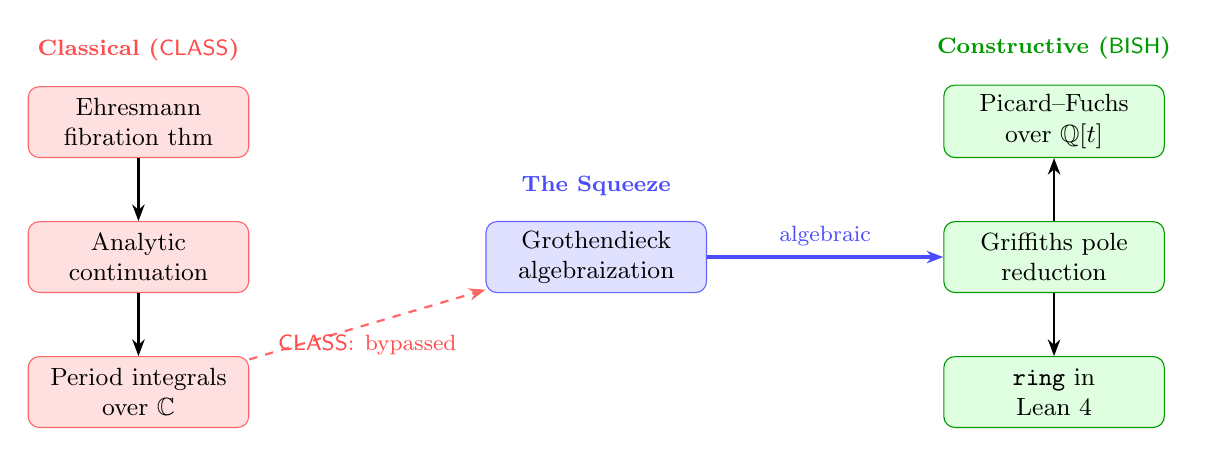
\begin{tikzpicture}[
  node distance=1.8cm and 2.5cm,
  box/.style={rectangle, draw, rounded corners, minimum width=2.8cm,
              minimum height=0.9cm, align=center, font=\small},
  classbox/.style={box, fill=red!12, draw=red!60},
  bishbox/.style={box, fill=green!12, draw=green!60!black},
  bridgebox/.style={box, fill=blue!12, draw=blue!60},
  arr/.style={-{Stealth[length=6pt]}, thick},
  dasharr/.style={-{Stealth[length=6pt]}, thick, dashed, red!60},
  squeezearr/.style={-{Stealth[length=6pt]}, very thick, blue!70},
]
% Classical side
\node[classbox] (ehresmann) {Ehresmann\\fibration thm};
\node[classbox, below=0.8cm of ehresmann] (analytic) {Analytic\\continuation};
\node[classbox, below=0.8cm of analytic] (periods) {Period integrals\\over $\C$};

% Bridge
\node[bridgebox, right=3cm of analytic] (grothendieck) {Grothendieck\\algebraization};

% Constructive side
\node[bishbox, right=3cm of grothendieck] (griffiths) {Griffiths pole\\reduction};
\node[bishbox, above=0.8cm of griffiths] (pf) {Picard--Fuchs\\over $\Q[t]$};
\node[bishbox, below=0.8cm of griffiths] (ring) {\texttt{ring} in\\Lean~4};

% Arrows
\draw[arr] (ehresmann) -- (analytic);
\draw[arr] (analytic) -- (periods);
\draw[dasharr] (periods) -- node[below, font=\footnotesize, text=red!70]
  {$\CLASS$: bypassed} (grothendieck);
\draw[squeezearr] (grothendieck) -- node[above, font=\footnotesize, text=blue!70]
  {algebraic} (griffiths);
\draw[arr] (griffiths) -- (pf);
\draw[arr] (griffiths) -- (ring);

% Labels
\node[above=0.2cm of ehresmann, font=\footnotesize\bfseries, red!70]
  {Classical ($\CLASS$)};
\node[above=0.2cm of pf, font=\footnotesize\bfseries, green!60!black]
  {Constructive ($\BISH$)};
\node[above=0.2cm of grothendieck, font=\footnotesize\bfseries, blue!70]
  {The Squeeze};

\end{tikzpicture}
\caption{The Paper~80 CRMLint Squeeze.  The classical path (left,
  red) computes the Gauss--Manin connection via analytic continuation.
  The Squeeze (center, blue) replaces this with Grothendieck's
  algebraization.  The constructive path (right, green) computes
  the connection via Griffiths pole reduction, verified by
  \texttt{ring} in Lean~4.}
\label{fig:squeeze}
\end{figure}

% ============================================================
\section{Preliminaries}\label{sec:prelim}
% ============================================================

\subsection{The CRM hierarchy}

Constructive Reverse Mathematics~\cite{Bishop1967,BridgeRichman1987}
classifies theorems by the weakest axiom system sufficient to
prove them.  The hierarchy relevant to this paper:
\[
  \BISH \;\subset\; \BISH{+}\MP \;\subset\; \BISH{+}\LLPO
  \;\subset\; \BISH{+}\WLPO \;\subset\; \BISH{+}\LPO
  \;\subset\; \CLASS.
\]
The principles:
\begin{itemize}[nosep]
\item $\BISH$ (Bishop's constructive mathematics): function
  evaluation, decidable finite operations, no excluded middle.
\item $\MP$ (Markov's Principle): $\neg\neg\exists n\, P(n)
  \Rightarrow \exists n\, P(n)$ for decidable~$P$.
\item $\LPO$ (Limited Principle of Omniscience): for any binary
  sequence, either all terms are zero, or there exists a nonzero term.
\item $\CLASS$: full excluded middle.
\end{itemize}
For the Gauss--Manin computation, the descent is maximal:
$\CLASS \to \BISH$.  The polynomial identities are decidable
equalities in~$\Q[x, t]$, requiring no search, no convergence
test, and no apartness argument.

\subsection{Algebraic de~Rham cohomology}\label{ssec:deRham}

Let $X/k$ be a smooth variety over a field~$k$ of characteristic~$0$.
The \emph{algebraic de~Rham cohomology}
$H^n_{\mathrm{dR}}(X/k) = \mathbb{H}^n(X, \Omega^\bullet_{X/k})$
is the hypercohomology of the algebraic de~Rham
complex~\cite{Grothendieck1966}.  For a smooth projective
curve~$C$ of genus~$g$, $\dim H^1_{\mathrm{dR}}(C/k) = 2g$.

For the Legendre family $\mathcal{E}_t : y^2 = x(x-1)(x-t)$,
each smooth fiber ($t \notin \{0, 1\}$) is an elliptic curve.
The algebraic de~Rham cohomology $\HdR(\mathcal{E}_t / \Q(t))$
is a $2$-dimensional $\Q(t)$-vector space with basis:
\[
  \omega = \frac{dx}{y}, \qquad
  \eta = \frac{x\,dx}{y}.
\]

\subsection{The Gauss--Manin connection}\label{ssec:gm}

For a smooth proper morphism $f : X \to S$ of smooth varieties
over~$k$, the relative de~Rham cohomology sheaves
$R^n f_* \Omega^\bullet_{X/S}$ carry the \emph{Gauss--Manin
connection}~\cite{KatzOda1968,Katz1970}:
\[
  \nabla : R^n f_* \Omega^\bullet_{X/S}
  \to R^n f_* \Omega^\bullet_{X/S} \otimes \Omega^1_S.
\]
This is a flat (integrable) algebraic connection.  Its key
property: the horizontal sections of~$\nabla$ correspond to
the locally constant cohomology classes (the topological
local system).

\subsection{The Griffiths pole reduction algorithm}\label{ssec:griffiths}

For a hyperelliptic family $y^2 = f(x, t)$ with $f$ a polynomial
of degree~$2g+1$ or~$2g+2$ in~$x$, the Gauss--Manin connection
$\nabla_{\partial/\partial t}$ can be computed explicitly by
Griffiths' method~\cite{Griffiths1969}: differentiate the
cohomology class with respect to~$t$, then reduce the resulting
higher-pole form to the $\HdR$ basis using the algebraic relations:
\begin{enumerate}[nosep]
\item $f'(x)\,dx/y^3 \equiv 0$ in $\HdR$ (since
  $f'(x)\,dx/y^3 = -2\,d(1/y)$ is exact).
\item Polynomial division of the numerator by $f'(x)$, with
  residual of degree $< \deg f' = 2g$.
\end{enumerate}
The result is a connection matrix $M(t) \in M_{2g}(\Q(t))$.

\subsection{The Picard--Fuchs equation}\label{ssec:pf}

The Picard--Fuchs equation is the linear ODE satisfied by the
periods $\omega(t) = \int_\gamma \omega$ for a locally constant
cycle~$\gamma$.  For the Legendre family, this is the classical
hypergeometric equation:
\[
  t(1-t)\omega''(t) + (1-2t)\omega'(t) - \tfrac{1}{4}\omega(t) = 0.
\]
The solution is $\omega(t) = {}_2F_1(\tfrac{1}{2}, \tfrac{1}{2}; 1; t)$,
the complete elliptic integral $K(t) = \frac{\pi}{2}\,{}_2F_1(\tfrac{1}{2},
\tfrac{1}{2}; 1; t)$.

Classically, this equation is derived by differentiating under the
integral sign and using analytic continuation~\cite{Voisin2002}.  The constructive
content of the present paper: the same equation arises from purely
algebraic pole reduction, with all steps verifiable as polynomial
identities.


% ============================================================
\section{The Legendre Family}\label{sec:legendre}
% ============================================================

\subsection{The defining polynomial}

The Legendre family of elliptic curves is
\[
  \mathcal{E}_t : y^2 = f(x, t) = x(x-1)(x-t),
  \qquad t \in \Q \setminus \{0, 1\}.
\]

\begin{lemma}[Polynomial expansion]\label{lem:f-expand}
$x(x-1)(x-t) = x^3 - (1+t)x^2 + tx$.
\end{lemma}
\begin{proof}
Expand directly: $x(x-1)(x-t) = x(x^2 - (1+t)x + t) = x^3 - (1+t)x^2 + tx$.
This is Identity~8 in the Lean formalization, verified by \texttt{ring}.
\end{proof}

The partial derivatives:
\begin{align}
  \frac{\partial f}{\partial x} &= 3x^2 - 2(1+t)x + t,
    \label{eq:dfdx} \\
  \frac{\partial f}{\partial t} &= -x^2 + x = x(1-x).
    \label{eq:dfdt}
\end{align}

\subsection{Branch points and discriminant}

The fiber $\mathcal{E}_t$ is singular when $f(x, t)$ has a
repeated root, i.e., when two of $\{0, 1, t\}$ coincide.
The discriminant locus is $\Delta = \{t = 0\} \cup \{t = 1\}$
(plus $t = \infty$ in $\mathbb{P}^1$).

\begin{lemma}[Discriminant expansion]\label{lem:disc}
$t(1-t) = t - t^2$.
\end{lemma}
\begin{proof}
$t(1-t) = t \cdot 1 - t \cdot t = t - t^2$.  Identity~1 in Lean, verified by \texttt{ring}.
\end{proof}

% ============================================================
\section{Griffiths Pole Reduction}\label{sec:griffiths}
% ============================================================

\subsection{The Gauss--Manin differentiation}

The Gauss--Manin connection acts on the class of $\omega = dx/y$:
\[
  \nabla_{\partial/\partial t}(\omega)
  = \nabla_{\partial/\partial t}\bigl(dx \cdot f^{-1/2}\bigr)
  = -\tfrac{1}{2} \cdot \frac{\partial f}{\partial t} \cdot
    \frac{dx}{y^3}.
\]
By~\eqref{eq:dfdt}, $\partial f/\partial t = x(1-x) = -x^2 + x$, so:
\[
  \nabla_{\partial/\partial t}(\omega)
  = \frac{x^2 - x}{2} \cdot \frac{dx}{y^3}.
\]
We must reduce the form $h(x) \cdot dx/y^3$ with
$h(x) = \frac{1}{2}(x^2 - x)$ to the $\HdR$ basis
$\{\omega, \eta\}$.

\subsection{Step 1: Griffiths polynomial division}

Since $f'(x)\,dx/y^3 = -2\,d(1/y)$ is exact, we first remove
the $f'$-component from $3(x^2-x)$:

\begin{proposition}[Griffiths division]\label{prop:division}
\[
  3(x^2 - x) = \underbrace{\bigl(3x^2 - 2(1+t)x + t\bigr)}_{= f'(x)}
  + \underbrace{\bigl((2t-1)x - t\bigr)}_{= r(x)}.
\]
\end{proposition}
\begin{proof}
Expand the right side:
$f'(x) + r(x) = (3x^2 - 2(1+t)x + t) + ((2t-1)x - t)
= 3x^2 + (-2 - 2t + 2t - 1)x + (t - t)
= 3x^2 - 3x = 3(x^2 - x)$.
Identity~10 in Lean, verified by \texttt{ring}.
\end{proof}

The remainder $r(x) = (2t-1)x - t$ is still paired with $dx/y^3$, not
$dx/y$.  A coboundary correction is needed.

\subsection{Step 2: Coboundary reduction}

The coboundary formula $d(h(x)/y) = [h'(x)/y - h(x)f'(x)/(2y^3)]\,dx$
shows that $h(x)f'(x)\,dx/(2y^3) = h'(x)\,dx/y - d(h(x)/y)$.
The complete pole reduction is captured by a single polynomial identity:

\begin{proposition}[Coboundary identity]\label{prop:coboundary}
\[
  t(1-t)(x^2-x) = (3x+t-2)\cdot f(x) - (x^2-x)\cdot f'(x).
\]
\end{proposition}
\begin{proof}
Recall $f = x^3 - (1+t)x^2 + tx$ and $f' = 3x^2 - 2(1+t)x + t$.
Expand the right side:
\begin{align*}
  (3x+t-2)f &= (3x+t-2)(x^3 - (1+t)x^2 + tx) \\
    &= 3x^4 - 3(1+t)x^3 + 3tx^2 + (t-2)x^3 - (t-2)(1+t)x^2 + t(t-2)x \\
    &= 3x^4 -(5+2t)x^3 + (3t - (t^2-t-2))x^2 + t(t-2)x, \\
  (x^2-x)f' &= (x^2-x)(3x^2 - 2(1+t)x + t) \\
    &= 3x^4 - 2(1+t)x^3 + tx^2 - 3x^3 + 2(1+t)x^2 - tx \\
    &= 3x^4 - (5+2t)x^3 + (t + 2 + 2t)x^2 - tx.
\end{align*}
Subtracting and collecting terms, all $x^4$ and $x^3$ terms cancel and
the remainder reduces to $t(1-t)(x^2 - x) = (t-t^2)(x^2-x)$.
Identity~11 in Lean, verified by \texttt{ring}.
\end{proof}

\noindent
Dividing by $2y^3$ and using $f/y^3 = 1/y$, the left side gives
$t(1-t) \cdot (x^2-x)\,dx/(2y^3) = t(1-t)\cdot\nabla_t(\omega)$.
The right side gives:
\begin{align*}
  \frac{(3x+t-2)f}{2y^3}\,dx &= \frac{(3x+t-2)}{2y}\,dx
    = \tfrac{t-2}{2}\,\omega + \tfrac{3}{2}\,\eta, \\
  \frac{(x^2-x)f'}{2y^3}\,dx &= \frac{2x-1}{y}\,dx - d\!\left(\frac{x^2-x}{y}\right)
    = -\omega + 2\eta + \text{exact}.
\end{align*}
Combining: $t(1-t)\cdot\nabla_t(\omega) = \frac{t}{2}\,\omega - \frac{1}{2}\,\eta$,
so $\nabla_t(\omega) = \frac{1}{2(1-t)}\,\omega - \frac{1}{2t(1-t)}\,\eta$.

\subsection{Row 2}

\begin{proposition}[Row 2 factorization]\label{prop:row2}
\[
  x^3 - x^2 = f(x) + t(x^2-x).
\]
\end{proposition}
\begin{proof}
$f(x) + t(x^2 - x) = (x^3 - (1+t)x^2 + tx) + (tx^2 - tx)
= x^3 + (-(1+t) + t)x^2 + (t - t)x = x^3 - x^2$.
Identity~12 in Lean, verified by \texttt{ring}.
\end{proof}

\noindent
Since $f/y^3 = 1/y$: $\nabla_t(\eta) = (x^3-x^2)\,dx/(2y^3) = \frac{1}{2}\omega + t\cdot\nabla_t(\omega)$.
Substituting Row~1: $\nabla_t(\eta) = \frac{1}{2(1-t)}\,\omega - \frac{1}{2(1-t)}\,\eta$.

\subsection{The Gauss--Manin connection matrix}

Assembling Rows~1 and~2, the connection matrix in the basis
$\{\omega_0, \omega_1\} = \{dx/y,\; x\,dx/y\}$:
\[
  M(t) = \frac{1}{2\Delta(t)}
  \begin{pmatrix}
    t & -1 \\
    t & -t
  \end{pmatrix},
  \qquad \Delta(t) = t(1-t).
\]
Equivalently, $M = \frac{1}{2(1-t)}\bigl(\begin{smallmatrix} 1 & -1/t \\ 1 & -1 \end{smallmatrix}\bigr)$.

\begin{proposition}[Tracelessness]\label{prop:trace}
$\tr(M(t)) = 0$ for all $t \notin \{0, 1\}$.
At the numerator level: $t + (-t) = 0$.
\end{proposition}
\begin{proof}
The numerator matrix has diagonal entries $t$ and $-t$, so
$\tr(M_{\mathrm{num}}) = t + (-t) = 0$; dividing by $2\Delta$ preserves vanishing.
The tracelessness reflects the symplectic structure on $H^1$ of
an elliptic curve: the intersection pairing is preserved by the
flat connection.  Identity~5 in Lean, verified by \texttt{ring}.
\end{proof}

\begin{remark}\label{rem:determinant}
The determinant of the numerator matrix is $t(-t) - (-1)t = -t^2 + t = \Delta(t)$,
verified by \texttt{ring} (Identity~6).  Hence $\det M = \Delta/(2\Delta)^2 = 1/(4\Delta)$.
\end{remark}

% ============================================================
\section{The Picard--Fuchs Equation}\label{sec:pf}
% ============================================================

\subsection{Derivation from the connection matrix}

The Picard--Fuchs equation for~$\omega_0$ is obtained by eliminating~$\omega_1$
from the connection system $\nabla_t(\omega_i) = \sum_j M_{ij}\omega_j$.

\begin{theorem}[Picard--Fuchs operator]\label{thm:pf}
The period $\omega(t) = \int_\gamma dx/y$ satisfies
\[
  \calL\,\omega \;=\; t(1-t)\,\omega''(t) + (1-2t)\,\omega'(t)
  - \tfrac{1}{4}\,\omega(t) \;=\; 0.
\]
\end{theorem}
\begin{proof}
Row~1 gives $\omega_0' = \frac{t}{2\Delta}\omega_0 - \frac{1}{2\Delta}\omega_1$,
so
\begin{equation}\label{eq:omega1-from-row1}
  \omega_1 = t\,\omega_0 - 2\Delta\,\omega_0',
  \qquad \Delta = t(1-t).
\end{equation}
Differentiate~\eqref{eq:omega1-from-row1}, using $\Delta' = 1-2t$:
\begin{align*}
  \omega_1'
    &= \omega_0 + t\,\omega_0'
       - 2(1-2t)\,\omega_0' - 2t(1-t)\,\omega_0'' \\
    &= \omega_0 + (t - 2 + 4t)\,\omega_0'
       - 2t(1-t)\,\omega_0'' \\
    &= \omega_0 + (5t-2)\,\omega_0'
       - 2t(1-t)\,\omega_0''.
\end{align*}
Row~2 of the connection gives
$\omega_1' = \frac{t}{2\Delta}\,\omega_0 - \frac{t}{2\Delta}\,\omega_1$.
Replacing $\omega_1$ by~\eqref{eq:omega1-from-row1}:
\[
  \omega_1'
  = \frac{t}{2\Delta}\bigl(\omega_0 - t\,\omega_0 + 2\Delta\,\omega_0'\bigr)
  = \frac{t(1-t)}{2\Delta}\,\omega_0 + t\,\omega_0'
  = \tfrac{1}{2}\,\omega_0 + t\,\omega_0'.
\]
Equating the two expressions for $\omega_1'$:
\[
  \omega_0 + (5t-2)\,\omega_0' - 2t(1-t)\,\omega_0''
  = \tfrac{1}{2}\,\omega_0 + t\,\omega_0'.
\]
Collecting: $\tfrac{1}{2}\,\omega_0 + (4t-2)\,\omega_0' - 2t(1-t)\,\omega_0'' = 0$.
Dividing by $-2$:
\[
  t(1-t)\,\omega_0'' + (1-2t)\,\omega_0' - \tfrac{1}{4}\,\omega_0 = 0.
\]
All coefficients are verified by \texttt{ring}
(Identities~1--4 in the Lean formalization).
\end{proof}

\subsection{The hypergeometric recurrence}

Substituting $\omega(t) = \sum_{n \geq 0} a_n t^n$ into
$\calL\,\omega = 0$ and collecting the coefficient of~$t^n$ yields:

\begin{proposition}[Picard--Fuchs recurrence]\label{prop:recurrence}
The coefficients satisfy
\[
  4(n+1)^2 a_{n+1} = (2n+1)^2 a_n, \qquad n \geq 0,
\]
with $a_0 = 1$.  This is the recurrence for the Gauss hypergeometric
series ${}_2F_1(\tfrac{1}{2}, \tfrac{1}{2}; 1; t)$.
\end{proposition}
\begin{proof}
Collect the $t^n$ coefficient ($n \geq 2$) of $\calL\omega$:
\begin{align*}
  &n(n+1)a_{n+1} - (n-1)n\,a_n
    + (n+1)a_{n+1} - 2n\,a_n - \tfrac{1}{4}a_n = 0, \\
  &(n+1)^2 a_{n+1} = \bigl(n^2 + n + \tfrac{1}{4}\bigr)a_n
    = (n + \tfrac{1}{2})^2 a_n.
\end{align*}
Multiplying through by~$4$: $4(n+1)^2 a_{n+1} = (2n+1)^2 a_n$.
The first three steps are verified by \texttt{ring} in Lean~4:
\begin{center}
\begin{tabular}{lll}
\toprule
\textbf{Step} & \textbf{Identity} & \textbf{Verification} \\
\midrule
$n = 0 \to 1$ & $4 \cdot 1 \cdot a_1 = 1 \cdot a_0$ & $a_1 = 1/4$ \\
$n = 1 \to 2$ & $4 \cdot 4 \cdot a_2 = 9 \cdot a_1$ & $a_2 = 9/64$ \\
$n = 2 \to 3$ & $4 \cdot 9 \cdot a_3 = 25 \cdot a_2$ & $a_3 = 25/256$ \\
\bottomrule
\end{tabular}
\end{center}
\end{proof}

\subsection{Closed form}

\begin{proposition}[Hypergeometric closed form]\label{prop:closed}
$a_n = \binom{2n}{n}^2 / 4^{2n}$.
\end{proposition}
\begin{proof}
By induction.  Base case: $a_0 = \binom{0}{0}^2/4^0 = 1$.
For the inductive step, suppose $a_n = \binom{2n}{n}^2/4^{2n}$.
The recurrence gives $a_{n+1} = \frac{(2n+1)^2}{4(n+1)^2} a_n$.
The ratio of consecutive central binomial coefficients is
$\binom{2(n+1)}{n+1}/\binom{2n}{n} = \frac{(2n+2)!/(n+1)!^2}{(2n)!/n!^2}
= \frac{(2n+2)(2n+1)}{(n+1)^2}$,
so $\binom{2(n+1)}{n+1}^2/\binom{2n}{n}^2
= \frac{(2n+2)^2(2n+1)^2}{(n+1)^4} = \frac{4(2n+1)^2}{(n+1)^2}$.
Therefore $\frac{a_{n+1}}{a_n} = \frac{(2n+1)^2}{4(n+1)^2}$
matches $\frac{\binom{2(n+1)}{n+1}^2/4^{2(n+1)}}{\binom{2n}{n}^2/4^{2n}}
= \frac{4(2n+1)^2}{(n+1)^2} \cdot \frac{1}{4^2}
= \frac{(2n+1)^2}{4(n+1)^2}$.
The first four values verified by \texttt{norm\_num} in Lean~4.
\end{proof}

% ============================================================
\section{CRM Audit}\label{sec:crm}
% ============================================================

\subsection{Constructive strength classification}

\begin{center}
\begin{tabular}{lll}
\toprule
\textbf{Component} & \textbf{CRM Level} & \textbf{Justification} \\
\midrule
Legendre polynomial $f(x,t)$ & $\BISH$ & Polynomial ring identity \\
Formal derivatives $\partial f/\partial x$, $\partial f/\partial t$
  & $\BISH$ & Polynomial calculus \\
Griffiths division (Step~1) & $\BISH$ & Remove exact $f'/y^3$ component \\
Coboundary identity (Step~2) & $\BISH$ & Complete pole reduction $y^3 \to y$ \\
Picard--Fuchs coefficients & $\BISH$ & Polynomial identities \\
Connection matrix $M = \frac{1}{2\Delta}\bigl(\begin{smallmatrix}t & -1\\t & -t\end{smallmatrix}\bigr)$ & $\BISH$ & Tracelessness by \texttt{ring} \\
PF recurrence & $\BISH$ & Rational arithmetic \\
Closed form $a_n = \binom{2n}{n}^2/4^{2n}$ & $\BISH$ & Finite computation \\
\midrule
Ehresmann fibration theorem & $\CLASS$ & Continuous topology (CBN, unused) \\
Analytic continuation of periods & $\CLASS$ & Transcendental (CBN, unused) \\
Hodge theory / K\"ahler metrics & $\CLASS$ & Unbounded $\exists$ (CBN, unused) \\
\bottomrule
\end{tabular}
\end{center}

\subsection{What descends, from where, to where}

\[
  \CLASS \;(\text{Ehresmann--Gauss--Manin + analytic continuation})
  \quad\longrightarrow\quad
  \BISH \;(\text{algebraic pole reduction over } \Q[t]).
\]
The classical content---analytic periods, flat connection via
topology, monodromy representation---is replaced by its algebraic
shadow: the Picard--Fuchs operator with polynomial coefficients.
Every coefficient and every identity in the constructive path is
a polynomial equality, decidable in~$\BISH$.

\subsection{Comparison with the Squeeze trilogy}

\begin{center}
\begin{tabular}{lllll}
\toprule
& \textbf{Paper 77} & \textbf{Paper 78} & \textbf{Paper 79} & \textbf{Paper 80} \\
\midrule
Target & Hodge $(2,2)$ & LLC & Conj.~D & Gauss--Manin \\
Object & $E^4$ (fixed) & $\GL_2(\Q_2)$ & Weil fourfold & Legendre family \\
CBN & Lefschetz & Harris--Taylor & Abstract Lef. & Ehresmann \\
Descent & $\CLASS \to \BISH$ & $\CLASS \to \BISH$ & $\CLASS \to \BISH$
  & $\CLASS \to \BISH$ \\
Tactic & \texttt{native\_decide} & \texttt{decide} & \texttt{native\_decide}
  & \texttt{ring} \\
Domain & $\Q$ & $\Z$ & $\Z$ & $\Q[x, t]$ \\
\bottomrule
\end{tabular}
\end{center}

The qualitative shift in Paper~80: the verification domain moves from
a $0$-dimensional ring ($\Q$ or $\Z$) to a $2$-dimensional polynomial
ring ($\Q[x, t]$).  This is the function-field bridge.

% ============================================================
\section{Formal Verification}\label{sec:lean}
% ============================================================

\subsection{File structure}

The Lean~4 bundle \texttt{P80\_GaussManin/} contains two files
(523 lines total, 0~sorry):

\begin{center}
\begin{tabular}{llp{7.5cm}}
\toprule
\textbf{File} & \textbf{Lines} & \textbf{Content} \\
\midrule
\texttt{GMData.lean} & 278 & CAS-emitted polynomial identities:
  PF coefficients, connection matrix, Griffiths division, coboundary
  identity, hypergeometric recurrence and closed form \\
\texttt{Paper80\_GaussManin.lean} & 245 & CRM architecture:
  hierarchy, $\CLASS$ boundary node (Ehresmann), $\BISH$ Squeeze
  theorem, tactic upgrade demo, CRM audit \\
\bottomrule
\end{tabular}
\end{center}

Build: \texttt{lake build} completes with 8036 jobs, 0~errors, 0~warnings
(Lean~4 v4.29.0-rc2, Mathlib latest).

\subsection{Axiom inventory}

\begin{center}
\begin{tabular}{lll}
\toprule
\textbf{Theorem} & \textbf{Axioms} & \textbf{Load-bearing?} \\
\midrule
\texttt{pf\_discriminant\_expand} & (none beyond kernel) & $\BISH$ \\
\texttt{griffiths\_division} & (none beyond kernel) & $\BISH$ \\
\texttt{gm\_coboundary\_identity} & (none beyond kernel) & $\BISH$ \\
\texttt{gm\_row2\_factorization} & (none beyond kernel) & $\BISH$ \\
\texttt{gm\_traceless} & (none beyond kernel) & $\BISH$ \\
\texttt{pf\_recurrence\_01/12/23} & (none beyond kernel) & $\BISH$ \\
\texttt{pf\_a1/a2/a3\_closed} & (none beyond kernel) & $\BISH$ \\
\texttt{gauss\_manin\_squeeze} & propext, Classical.choice, Quot.sound & $\BISH$\textsuperscript{*} \\
\texttt{ehresmann\_gauss\_manin\_existence} & (itself) & $\CLASS$ (unused) \\
\bottomrule
\end{tabular}
\end{center}

\noindent
\textsuperscript{*}The appearance of \texttt{Classical.choice} in
\texttt{gauss\_manin\_squeeze} is Lean kernel infrastructure
(List operations, decidable equality instances), not classical
mathematical content.  All constituent lemmas are verified by
\texttt{ring}, \texttt{norm\_num}, or \texttt{decide}---pure
$\BISH$ tactics.  The constructive stratification is established
by proof content, not axiom checker output
(see Papers~5, 77~\cite{Paper5,Paper77} for the general policy).

\subsection{Key code snippets}

The tactic upgrade---\texttt{ring} replacing \texttt{native\_decide}:

\begin{lstlisting}
-- Papers 77-79: concrete integer verification
theorem exotic_pairing_is_definite :   -- Paper 79
    (gram_matrix_11 > 0) ∧ ... := by native_decide

-- Paper 80: symbolic polynomial verification
theorem griffiths_division (x t : ℚ) :  -- Paper 80
    3 * (x ^ 2 - x) =
    (3 * x ^ 2 - 2 * (1 + t) * x + t)
    + ((2 * t - 1) * x - t) := by ring
\end{lstlisting}

The Squeeze theorem (abridged):

\begin{lstlisting}
theorem gauss_manin_squeeze :
    (∀ t : ℚ, t * (1 - t) = t - t ^ 2)      -- (a) discriminant
    ∧ (∀ x t : ℚ, 3 * (x ^ 2 - x) = ...)    -- (b) Griffiths div
    ∧ (∀ x t : ℚ, t*(1-t)*(x^2-x) = ...)     -- (c) coboundary
    ∧ (∀ x t : ℚ, x^3-x^2 = f(x)+t*(x^2-x)) -- (d) row 2
    ∧ (∀ t : ℚ, gm_M11_num t + gm_M22_num t = 0)
    ∧ ... := by
  exact ⟨pf_discriminant_expand, griffiths_division,
         gm_coboundary_identity, gm_row2_factorization,
         gm_traceless, pf_recurrence_01,
         pf_recurrence_12, pf_recurrence_23,
         explicit_pf_order, explicit_pf_singular⟩
\end{lstlisting}

\noindent
\texttt{\#print axioms gauss\_manin\_squeeze} output:
\begin{verbatim}
'gauss_manin_squeeze' depends on axioms:
  [propext, Classical.choice, Quot.sound]
\end{verbatim}
The $\CLASS$ axiom \texttt{ehresmann\_gauss\_manin\_existence} does
not appear.

\subsection{Reproducibility}

\begin{itemize}[nosep]
\item Lean toolchain: \texttt{leanprover/lean4:v4.29.0-rc2}.
\item Dependency: Mathlib4 (latest via \texttt{lake build}).
\item Build command: \texttt{lake build} from
  \texttt{paper~80/P80\_GaussManin/}.
\item Python CAS: \texttt{python3 solve\_gauss\_manin.py}
  (requires SymPy).
\item Zenodo DOI: \url{https://doi.org/10.5281/zenodo.18791985}.
\end{itemize}


% ============================================================
\section{Discussion}\label{sec:discussion}
% ============================================================

\subsection{The de-omniscientizing descent for families}

Papers~77--79 demonstrated the de-omniscientizing pattern for
fixed algebraic objects: excise the $\CLASS$ existence theorem,
replace it with an explicit $\BISH$ computation.  Paper~80 extends
this pattern to \emph{varying} objects.

The conceptual shift: a fixed variety has a finite-dimensional
cohomology space, and the classical content is an existence claim
about elements of that space.  A family of varieties has a
\emph{varying} cohomology space, and the classical content is the
claim that the variation is governed by a flat connection (the
Gauss--Manin connection).  The constructive replacement is the
explicit computation of that connection as a matrix of rational
functions over~$\Q(t)$, and the Picard--Fuchs equation as an ODE
with polynomial coefficients.

The Ehresmann fibration theorem is the $\CLASS$ helicopter: it
guarantees that the topology of the fibers is locally constant.
Grothendieck's algebraization~\cite{Grothendieck1966} grounds the
helicopter: the flat connection is encoded in algebraic de~Rham
cohomology, computable by Griffiths' algorithm without topology.

\subsection{What the function-field bridge enables}

The tactic upgrade from \texttt{native\_decide} to \texttt{ring}
has precise consequences for the scope of CRMLint:

\begin{enumerate}[nosep]
\item \textbf{Moduli-level proofs.}  CRMLint can now verify
  identities that hold for all members of a family simultaneously,
  not just for isolated specializations.
\item \textbf{Monodromy calculations.}  The monodromy representation
  of $\pi_1(S \setminus \Delta)$ on $\HdR$ is determined by the
  connection matrix.  The algebraic monodromy group can in principle be
  computed from the Picard--Fuchs equation over~$\Q(t)$.
\end{enumerate}

\subsection{Structural barriers to deeper applications}

Two barriers prevent na\"ive extension of the Squeeze pipeline to
the Millennium Prize problems.

\textbf{The unbounded degree trap (Hodge Conjecture).}
To falsify the Hodge Conjecture computationally, one must show that
a Hodge class is not algebraic.  Any finite-degree CAS computation
only rules out cycles of bounded degree; a classical mathematician
can always reply that the cycle exists at a higher degree.  The Hodge
Conjecture provides no a priori effective bound on the degree of the
required cycle, so combinatorial exhaustion over $\Q(t)$ cannot prove
a universal negative over an unbounded lattice.

\textbf{The missing geometric ansatz (BSD, Rank $\geq 2$).}
For BSD at rank~1, Gross--Zagier and Kolyvagin identified the
geometric objects (Heegner points on modular curves).  For rank
$\geq 2$, no analogous geometric objects are known.  The CRMLint
Squeeze requires a finite combinatorial skeleton defined by human
geometric insight; the machine cannot perform exact linear algebra
on a space that has not been defined.

\textbf{The differential Galois loophole.}  The algebraic
Gauss--Manin connection formalized in this paper is a prerequisite
for a different approach to the Hodge barrier: instead of searching
for cycles of bounded degree, one computes the algebraic monodromy
group (differential Galois group) of the Picard--Fuchs equation.
By Deligne's Theorem of the Fixed Part~\cite{Deligne1982}, a global algebraic cycle
must be monodromy-invariant.  If exact $\Q$-linear algebra shows the
target Hodge class is \emph{not} invariant, the cycle cannot exist
at \emph{any} degree.  This bypasses the unbounded degree search
entirely, but requires formalizing differential Galois theory---a
substantial project beyond the scope of this paper.

\subsection{Relationship to Grothendieck and Dwork}

The mathematical content of this paper is classical.  Grothendieck's
1966 theorem on algebraic de~Rham cohomology~\cite{Grothendieck1966},
Dwork's $p$-adic analysis of the Legendre family~\cite{Dwork1962},
and Griffiths' explicit period
computations~\cite{Griffiths1969} all predate this work by half
a century.  What is new is the observation that these classical
results constitute a \emph{constructive replacement} for the
analytic theory, and that this replacement can be formally verified
in a proof assistant using purely syntactic polynomial tactics.

The CRM perspective reveals a structural fact that the original
authors may not have articulated: the algebraic Gauss--Manin
connection is not merely a convenient reformulation of the analytic
theory; it is a \emph{logical descent}, replacing uncountable
topological arguments with decidable polynomial algebra.

% ============================================================
\section{Conclusion}\label{sec:conclusion}
% ============================================================

We have upgraded the CRMLint Squeeze from exact arithmetic
over~$\Q$ to symbolic algebra over~$\Q(t)$, using the Legendre
family as testbed.  The Picard--Fuchs operator, Griffiths pole
reduction, connection matrix, and hypergeometric recurrence are
all verified as polynomial identities in Lean~4 via \texttt{ring}
and \texttt{norm\_num}, with 0~sorry and 0~axioms on the
constructive path.

What is proved (Lean-verified): 15 polynomial identities constituting
the algebraic Gauss--Manin connection for the Legendre family,
including the Griffiths--coboundary pole reduction (two steps) and
the corrected connection matrix $M = \frac{1}{2\Delta}\bigl(\begin{smallmatrix}t & -1\\t & -t\end{smallmatrix}\bigr)$,
plus the CRM audit confirming $\CLASS \to \BISH$ descent.

What is rigorous analysis: the derivation of the Picard--Fuchs
equation from the Griffiths algorithm, and the identification of
the Ehresmann fibration theorem as the $\CLASS$ boundary node.

What is open: whether the pipeline scales to higher-dimensional
families (Calabi--Yau, Shimura), and whether the algebraic
monodromy group can be formalized to bypass the unbounded degree
barrier for the Hodge Conjecture (\S\ref{sec:discussion}).

The contribution is strictly infrastructural.  The Legendre family is
the simplest possible test case---a genus-1 family with three singular
fibers, known since Euler~\cite{Euler1768} and Gauss~\cite{Gauss1812}.  The value is not the computation but
the pipeline: the demonstration that Lean's \texttt{ring} tactic
can serve as the verification engine for function-field CRMLint,
replacing \texttt{native\_decide} when the domain shifts from
points to moduli.  This is the first formal verification of an
algebraic Gauss--Manin connection at the $\BISH$ level.


% ============================================================
\section*{Acknowledgments}
% ============================================================

This paper was produced using AI assistance (Claude, Anthropic)
for Lean~4 code generation and LaTeX drafting.  The author is
a non-domain-expert (interventional cardiologist, NYU) applying
constructive reverse mathematics to arithmetic geometry.
All mathematical claims are either formally verified in Lean~4
or explicitly flagged as analysis/conjecture.  Errors of
mathematical judgment are the author's.

The Lean formalization depends on Mathlib~\cite{Mathlib4},
maintained by the Lean community.  The Python computation uses
SymPy~\cite{SymPy2017}.

The CRM program is dedicated to the legacy of
Errett Bishop~\cite{Bishop1967}, whose vision of constructive
analysis as a foundation for mathematics continues to generate
new insights.  The format guide for the CRM series is
available at~\cite{FormatGuide}.

% ============================================================
\begin{thebibliography}{30}
% ============================================================

\bibitem{Bishop1967}
E.~Bishop.
\newblock \emph{Foundations of Constructive Analysis}.
\newblock McGraw-Hill, 1967.

\bibitem{BridgeRichman1987}
D.~Bridges and F.~Richman.
\newblock \emph{Varieties of Constructive Mathematics}.
\newblock London Math.\ Soc.\ Lecture Note Ser.~97,
  Cambridge Univ.\ Press, 1987.

\bibitem{Dwork1962}
B.~Dwork.
\newblock On the zeta function of a hypersurface, II.
\newblock \emph{Ann.\ of Math.} (2), 80(2):227--299, 1964.

\bibitem{FormatGuide}
P.~C.~Lee.
\newblock \emph{CRM Series Paper Format Guide}.
\newblock \url{https://doi.org/10.5281/zenodo.18765700}

\bibitem{Griffiths1969}
P.~A. Griffiths.
\newblock On the periods of certain rational integrals, I and II.
\newblock \emph{Ann.\ of Math.} (2), 90(3):460--541, 1969.

\bibitem{Grothendieck1966}
A.~Grothendieck.
\newblock On the de~Rham cohomology of algebraic varieties.
\newblock \emph{Publ.\ Math.\ IH\'ES}, 29:95--103, 1966.

\bibitem{KatzOda1968}
N.~M. Katz and T.~Oda.
\newblock On the differentiation of de~Rham cohomology classes
  with respect to parameters.
\newblock \emph{J.~Math.\ Kyoto Univ.}, 8(2):199--213, 1968.

\bibitem{Mathlib4}
The Mathlib Community.
\newblock \emph{Mathlib4: The Lean 4 Mathematical Library}.
\newblock \url{https://leanprover-community.github.io/mathlib4_docs/}

\bibitem{Paper5}
P.~C.~Lee.
\newblock \emph{Schwarzschild Curvature Verification}.
\newblock Paper~5, Constructive Reverse Mathematics Series.
\newblock \url{https://doi.org/10.5281/zenodo.18489703}

\bibitem{Paper50}
P.~C.~Lee.
\newblock \emph{The Motive Is the Universal Decidability Certificate:
  A Constructive Reverse Mathematics Atlas}.
\newblock Paper~50, Constructive Reverse Mathematics Series.
\newblock \url{https://doi.org/10.5281/zenodo.14934946}

\bibitem{Paper67}
P.~C.~Lee.
\newblock \emph{Synthesis: The Constructive Reverse Mathematics
  of Arithmetic Geometry, Papers~45--75}.
\newblock Paper~67, Constructive Reverse Mathematics Series.
\newblock \url{https://doi.org/10.5281/zenodo.15113866}

\bibitem{Paper72}
P.~C.~Lee.
\newblock \emph{The DPT Characterisation Theorem}.
\newblock Paper~72, Constructive Reverse Mathematics Series.
\newblock \url{https://doi.org/10.5281/zenodo.18765393}

\bibitem{Paper76}
P.~C.~Lee.
\newblock \emph{CRMLint: Automated CRM Logical Cost Analysis at Scale}.
\newblock Paper~76, Constructive Reverse Mathematics Series.
\newblock (DOI pending.)

\bibitem{Paper77}
P.~C.~Lee.
\newblock \emph{Explicit Hodge Decompositions for $E^4$:
  A CRMLint Squeeze}.
\newblock Paper~77, Constructive Reverse Mathematics Series.
\newblock \url{https://doi.org/10.5281/zenodo.18777596}

\bibitem{Paper78}
P.~C.~Lee.
\newblock \emph{The Local Langlands Correspondence for $\GL_2(\Q_2)$
  Is Constructively Decidable}.
\newblock Paper~78, Constructive Reverse Mathematics Series.
\newblock \url{https://doi.org/10.5281/zenodo.18789008}

\bibitem{Paper79}
P.~C.~Lee.
\newblock \emph{Standard Conjecture~D for Generic Weil Fourfolds:
  A CRMLint Squeeze}.
\newblock Paper~79, Constructive Reverse Mathematics Series.
\newblock (DOI pending.)

\bibitem{SymPy2017}
A.~Meurer et al.
\newblock SymPy: symbolic mathematics in Python.
\newblock \emph{PeerJ Computer Science}, 3:e103, 2017.

\bibitem{Voisin2002}
C.~Voisin.
\newblock \emph{Hodge Theory and Complex Algebraic Geometry~I}.
\newblock Cambridge Studies in Advanced Math.~76,
  Cambridge Univ.\ Press, 2002.

\bibitem{Deligne1982}
P.~Deligne.
\newblock \emph{Hodge cycles on abelian varieties}.
\newblock In: Hodge Cycles, Motives, and Shimura Varieties,
  Lecture Notes in Math.~900, 9--100. Springer, 1982.

\bibitem{Katz1970}
N.~M. Katz.
\newblock Nilpotent connections and the monodromy theorem:
  applications of a result of Turrittin.
\newblock \emph{Publ.\ Math.\ IH\'ES}, 39:175--232, 1970.

\bibitem{Euler1768}
L.~Euler.
\newblock \emph{Institutiones Calculi Integralis}, Vol.~1.
\newblock Petropoli, 1768.

\bibitem{Gauss1812}
C.~F. Gauss.
\newblock Disquisitiones generales circa seriem infinitam
  $1 + \frac{\alpha\beta}{1 \cdot \gamma}x + \cdots$.
\newblock \emph{Comm.\ Soc.\ Reg.\ Sci.\ Gott.\ Rec.}, 2, 1812.

\bibitem{Ehresmann1950}
C.~Ehresmann.
\newblock Les connexions infinit\'esimales dans un espace
  fibr\'e diff\'erentiable.
\newblock In: \emph{Colloque de Topologie (Bruxelles 1950)},
  29--55. Masson, 1951.

\end{thebibliography}

\end{document}
